\documentclass[a4paper,12pt]{article} % тип документа

% report, book



%  Русский язык

\usepackage[T2A]{fontenc}			% кодировка
\usepackage[utf8]{inputenc}			% кодировка исходного текста
\usepackage[english,russian]{babel}	% локализация и переносы
\usepackage{graphicx}
\graphicspath{{./}}
\DeclareGraphicsExtensions{.png,.jpg}


% Математика
\usepackage{amsmath,amsfonts,amssymb,amsthm,mathtools} 


\usepackage{wasysym}

%Заговолок
\author{Бредихин Александр}
\title{Домашняя работа №3}



\begin{document} % начало документа

\maketitle

\subsection*{Задача 1}
\textit{Задача:} язык 2-COLOR состоит из кодировок всех графов, заданных матрицами смежности, вершины которых можно корректно окрасить в два цвета (никакие две смежные вершины не имеют один цвет). Верно ли, что язык 2-COLOR лежит в $\mathcal{P}$? В $\mathcal{NP}$? В $co-\mathcal{NP}$?\\

Построим алгоритм, которое за полиномиальное время будет определять, можно ли правильно раскрасить данный граф, который подаётся матрицей смежности, в два цвета (пусть $ n $ -- количество вершин в графе) (алгоритм построен на приципе обхода графа в ширину)\\

Алгоритм: 
\begin{itemize}
\item[1)] Выбираем произвольную непокрашенную вершину графа и красим её в цвет с номером $ 0 $ (в любой из двух цветов: 0 или 1)
\item[2)] По матрице смежности смотрим на все смежные вершины с выбранной: если смежная вершина непокрашена ни в какой цвет, красим её в противоположный и добавляем в стек, если она уже покрашена в противоположный цвет, то не изменяем его, и вершину тоже добавляем в стек. Если смежная вершина уже окрашена в такой же цвет, то заканчиваем алгоритм. Это говорит, что в графе есть цикл нечётной длины и то, что нельзя правильно раскрасить граф в 2 цвета.\\
Также создаём массив просматренных вершин, куда добавляем каждую вершину после проверки всех вершин ей смежных. В стек добавляем только если этой вершины нет в массиве просмотренных (чтобы не возникло зацикливания)
\item[3)] Для каждой из вершин в стеке запускаем пункт 2 пока стек не будет пустым. Если все вершины в графе попали в массив просмотренных и алгоритм не завершился досрочно, то мы получили правильную раскраску графа в 2 цвета. Если какая-то вершина не попала в массив просмотренных, то в графе несколько компонент связности и запускаем пункт 1 от этой вершины.
\end{itemize}
Коректность понятна, так как каждые смежные вершины нужно красить в разные цвета, что и делает алгоритм. Алгоритм проходит все вершины по одному разу и проверяет по матрице смежности все смежные с ней вершины. Следовательно, грубо сложность можно оценить как $ O(n^2) $\\
Получили алгоритм, решающий задачу 2-COLOR за полиноминальное время $ \longrightarrow $ 2-COLOR лежит в $\mathcal{P}$ $ \longrightarrow $ лежит в $\mathcal{NP}$ и в $co-\mathcal{NP}$


\subsection*{Задача 2}
\textit{Задача:} язык $HP$ состоит из всех графов, имеющих гамильтонов путь (несамопересекающийся путь, проходящий через все вершины графа). Язык $HC$ состоит из всех графов, имеющих гамильтонов цикл (цикл, проходящий через все вершины, в котором все вершины, кроме первой и последней, попарно различны).
Постройте явные полиномиальные сводимости $HC$ к $HP$ и наоборот.\\

Сводимость: $ HC \leq_p HP $, \\
то есть нужно построить функцию $ f $, такую что $ x \in HC \Longleftrightarrow f(x)\in HP $
Пусть функция $ f $ по данному ей графу делает следующее:
\begin{itemize}
\item[1] Выбирает произвольную вершину графа (назовём её $ A $) и дублирует её -- $ A^* $.
\item[2] Проводит рёбра от вершины $ A^* $ ко всем вершинам, с которыми соединена $ A $.
\item[3] Создаёт ещё 2 вершины $ M $ и $ N $ и соединяет одну из них с $ A $ (б.о.о. вершину $ M $), а другую с $ A^* $
\end{itemize}

Пусть граф $ x \in HC $, покажем что в созданном графе $ f(x) $ будет гамильтонов путь: начинаем из вершины $ M $ переходим в вершину $ A $ а затем идём по гамильтонову циклу (так как $ x \in HC $, то в графе без вершин $ M,N,A^* $ он существует). Когда доходим до вершины которя соединена с $ A $ (и при этом мы уже обошли все вершины графа $ x $), то идём в вершину $ A^* $ и затем в $ N $. Получили гамильтонов путь, так как прошли по всем вершинам графа $ f(x) $ без самопересечений $ \longrightarrow f(x)\in HP$

Пусть граф $ x \notin HC $, покажем, что у графа $ f(x) $ не будет гамильтонова пути: от противного, пусть в $ f(x) $ есть гамильтонов путь, тогда он точно начинается или заканчивается в вершинах $ M $ и $ N $ (так как они висячие) $ \longrightarrow $ в $ f(x) $ без этих двух вершин есть гамильтонов путь, но тогда в $ x $ есть гамильтонов цикл, так как последний переход гамильтонова пути в графе $ f(x) $ без $ M $ и $ N $ можно заменить на переход в вершину $ A $ (то есть замкнуть гамильтонов путь и получить гамильтонов цикл в $ x $). Получили противоречие, что $ x \notin HC \longrightarrow$ в $ f(x) $  нет гамильтонова пути.

Функция $ f $ -- полиномиальна, так как мы достраиваем только 3 вершины и проводим $ n-1 + 1 + 1 $ ребро (можно сказать добавляем в матрицу смежности 3 строки, это полином)\\



Сводимость: $ HP \leq_p HC $, \\
то есть нужно построить функцию $ f $, такую что $ x \in HP \Longleftrightarrow f(x)\in HС $.
Пусть функция $ f(x) $ по данному графу делает следующие: создаёт вершину (назовём её $ A $) и проводит из этой вершины рёбра ко всем вершинам графа $ x $

Пусть $ x\in HP $, покажем, что тогда в графе $ f(x) $ найдётся гамильтонов цикл. Так как  $ x\in HP \longrightarrow$
в графе $ x $ есть гамильтонов путь, который начинается в вершине $ B $ и заканчивается в вершине $ C $. Тогда идя из вершины $ A $ графа $ f(x) $ в вершину $ B $, затем по обозначенному гамельтонову пути в $ D $ и затем из $ D $ в $ A $ получим гамильтонов цикл (прошли все вершины графа и нигде кроме вершины $ A $ не было самопересечений)

Пусть  $ x\notin HP $, покажем, что тогда в графе $ f(x) $ НЕ найдётся гамильтонова цикла. От противного, пусть он есть, следовательно он проходит через вершину $ A $ и все вершины графа $ x $. Пусть в $ A $ этот цикл попадает из вершины $ B $ а затем идёт в вершину $ C $, тогда путь из вершины $ B $ в $ C $ гамильтоновый для графа $ x $ (так как проходит через все его вершины и нигде не пересекается (получен из гамильонова цикла <<удалением>> добавленной вершины)). Получаем противоречие $ \longrightarrow $ $ f(x)\notin HC $
\subsection*{Задача 4}
Задача: докажите следующие свойства полиномиальной сводимости:
($i$) Рефлексивность: $A\leq_p A$; транзитивность: $A\leq_p B, B\leq_p C \implies A\leq_p C$;\\
($ii$) Если $B\in\mathcal{P}$ и $A\leq_p B$, то $A\in\mathcal{P}$;\\
($iii$) Если $B\in\mathcal{NP}$ и $A\leq_p B$, то $A\in\mathcal{NP}$.\\

P.S. задача была разобрана на лекции 

{\bf ($i$)} Рефлексивность (то есть $ A \leq_p A) $): рассмотрим функцию $ f(x) = x $ (очевидно, что тогда будет выполняться утверждение $ x \in A \Longleftrightarrow f(x)\in A $)

Транзитивность (то есть $A\leq_p B, B\leq_p C \implies A\leq_p C$): рассмотрим функцию $ f $ как композицию $ f = h \circ g $, где $ h $ сводит $ A $ к $ B $, а $ g $ сводит $ B $ к $ C $. Получается: если $ x\in A \Leftrightarrow h(x)\in B \Leftrightarrow f(x) = g(h(x))\in C $. И так как $ h $ и $ g $ -- полиномиально вычислимы, то $ h \circ g $ также вычисляется за полиномиальное время.

{\bf ($ii$)} Так как $B\in\mathcal{P}$, то $ \exists \chi_{B}$ -- характеристическая функция языка $ B $ (говорит за полиномиальное время лежит произвольный $ x $ в языке $ B $ или нет). Так как $A\leq_p B \longrightarrow \exists f \text{-полиномиальная} :x \in A \Longleftrightarrow f(x)\in B $. \\
Рассмотрим функцию $ \chi_A = f \circ \chi_{B} $, она является характеристической функцией для $ A $, так как $x \in A \Leftrightarrow f(x) \in B \Leftrightarrow \chi_B(f(x)) = 1$. Аналогично предыдущему пункту, так как $ f $, $ \chi_B $ -- полиномиальны, следовательно их композиция вычисляется тоже за полиномиальное время (то есть характеристическая функция для $A$ вычисляется за полиномиальное время) $ \longrightarrow  A\in\mathcal{P}$

{\bf ($iii$)} Аналогично предыдущему пункту, только теперь $ \chi_B $ -- вычисяляется на недетерменированной МТ (так как $B\in\mathcal{NP}$). $\chi_{A}=\chi_{B} \circ f$ -- является характерестической функцией для языка $ A $ и вычисляется за полиномиальное время на недетременнированной МТ (так как $ f $ - полиномиальная даже на детерменированной МТ) $ \longrightarrow$ по определению $ \mathcal{NP} \Rightarrow$ $A\in\mathcal{NP}$

\subsection*{Задача 5}
Докажите, что классы $\mathcal{P}$ и $\mathcal{NP}$ замкнуты относительно \\
операции $*$~---~звезды Клини (была в ТРЯПе). Приведите также и сертификат принадлежности слова языку $L^*$, где $L\in\mathcal{NP}$. \\

для $\mathcal{P}$\\
Пусть $ p $ - характеристическая функция языка $ L $, построим характеристическую функцию $ q $ для языка $L^*$. Ниже представлен псевдокод, который реализует её:
\begin{center}
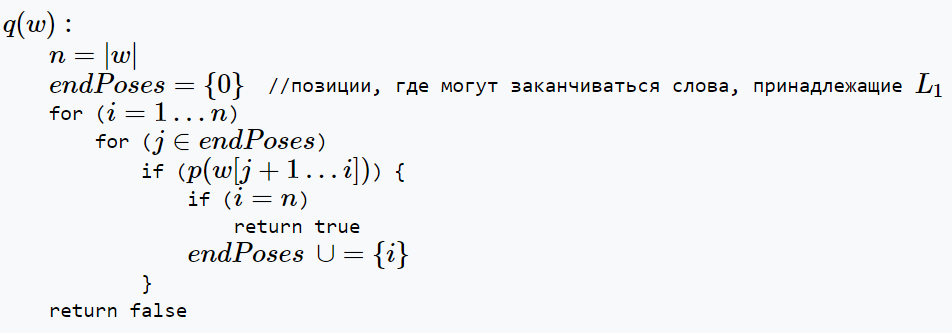
\includegraphics[width=0.7\textwidth]{Code}
\end{center}

Алгоритм: \\
в цикле по входному слову $ w $ провереят с помощью характеристической функции для языка $ L $ -- $ p $ принадлежит ли подслово языку. Для этого создаём массив $ END $, который первоначально пуст и кладём туда индексы концов слов, которые разбиваются на подслова из $ L $ (для этого для каждого индекса из $ END $ и текущего значения $ i $ берём слайс от входного слова и проверяем из $ L $ оно или нет: если из $ L $, то добавляем $ i $ в массив $ END $, что говорит что подслово $ w $ до этого элемента может быть получено конкатинацией слов из $ L $)\\
Цикл завершается, когда $ i == len(w) $. Если $ \exists j\in END: w[j+1,n+1]\in L \longrightarrow w\in L^* $, и выводится 1, иначе слово $ w $ не разбивается на подслова из $ L \longrightarrow \notin L^* $\\
Количество элементов в массиве $ END $ не может быть больше, чем $ n $ (длина входного слова). Следовательно в худшем случае, так как есть цикл в цикле, сложность оценивается $ O(n^2) $ -- полином. Следовательно, мы получили полиномиальную характеристическую функцию для $ L^* $, значит $ L^* \in \mathcal{P} $

для $\mathcal{NP}$\\
$ L\in \mathcal{NP} \longrightarrow \exists \text{ предикат } R_L(x, y) $. Построим предикат для $ L^* $. Для этого предикату $R_L^*$ в качестве подсказки (сертификата) подаём начала слов из $ L $ и подсказки для каждого из этих слов. Тогда предикат $R_L^*$ запускает предикат $R_L$ на каждом подслове и переданной для неё подсказкой. $R_L^*$ выдаёт 1, когда на всех подславах предикат для $ L $ выдал 1, иначе 0.\\
Подсказка полиномиальна от длины входного слова (количество индексов разбиения не может превышать длины входного слова). $ R_L $ выполняется полиномиально и не может быть запущен ,чем $ n $ раз, следовательно мы построили полиномиальный предикат для $ L^* $.
\end{document} % конец документа